\chapter{K vecinos más próximos}\label{Chapter5} 
% chktex-file 8
% chktex-file 12
% chktex-file 13
% chktex-file 44

En teoría, siempre se desearía predecir respuestas cualitativas usando el clasificador de Bayes. Pero para datos reales, no se conoce la distribución condicional de $Y$ dado $X$, por lo que calcular el clasificador de Bayes es imposible. Por lo tanto, el clasificador de Bayes sirve como un estándar inalcanzable contra el cual comparar otros métodos. Muchos enfoques intentan estimar la distribución condicional de $Y$ dado $X$, y luego clasificar una observación dada a la clase con la mayor probabilidad estimada. Uno de estos métodos es el clasificador de $K$-vecinos más próximos (KNN). Sea un entero positivo $K$ y una observación de prueba $x_0$, el clasificador KNN primero identifica los $K$ puntos en los datos de entrenamiento que están más cerca de $x_0$, representados por $\mathcal{N}_0$. Luego estima la probabilidad condicional para la clase $j$ como la fracción de puntos en $\mathcal{N}_0$ cuyos valores de respuesta son iguales a $j$:
\begin{equation}
\Pr(Y = j | X = x_0) = \frac{1}{K} \sum_{i \in \mathcal{N}_0} I(y_i = j)
\label{eq:2.12}
\end{equation}

Finalmente, KNN aplica la regla de Bayes y clasifica la observación de prueba $x_0$ a la clase con la mayor probabilidad. \\

\begin{figure}[h]
\centering
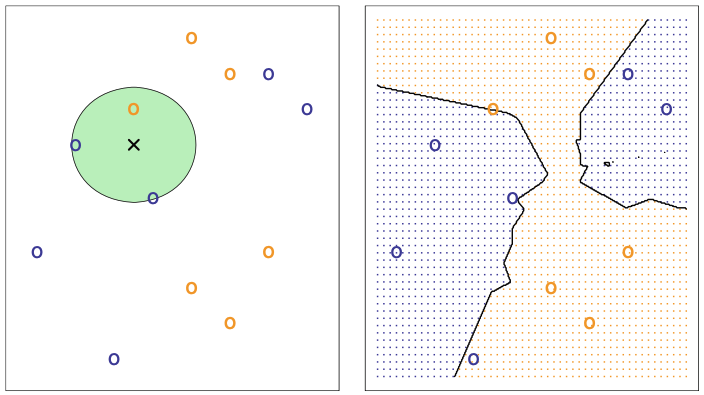
\includegraphics[width=0.6\textwidth]{fotos/10.png}
\caption{El enfoque KNN, usando $K = 3$, se ilustra en una situación simple con seis observaciones azules y seis observaciones naranjas. Izquierda: una observación de prueba para la cual se desea una etiqueta de clase predicha se muestra como una cruz negra. Se identifican los tres puntos más cercanos a la observación de prueba, y se predice que la observación de prueba pertenece a la clase que ocurre con mayor frecuencia, en este caso azul. Derecha: La frontera de decisión KNN para este ejemplo se muestra en negro. La cuadrícula azul indica la región en la cual una observación de prueba será asignada a la clase azul, y la cuadrícula naranja indica la región en la cual será asignada a la clase naranja.}
\label{fig:2.14}
\end{figure}

La figura \ref{fig:2.14} proporciona un ejemplo del enfoque KNN. En el panel izquierdo, se ha graficado un pequeño conjunto de datos de entrenamiento que consiste en seis observaciones azules y seis naranjas. El objetivo es hacer una predicción para el punto etiquetado con la cruz negra. Supongamos que se elige $K = 3$. Entonces KNN primero identificará las tres observaciones que están más cerca de la cruz. Este vecindario se muestra como un círculo. Consiste en dos puntos azules y un punto naranja, resultando en probabilidades estimadas de $2/3$ para la clase azul y $1/3$ para la clase naranja. Por lo tanto, KNN predecirá que la cruz negra pertenece a la clase azul. En el panel derecho de la figura \ref{fig:2.14} se ha aplicado el enfoque KNN con $K = 3$ en todos los valores posibles para $X_1$ y $X_2$, y se ha dibujado la correspondiente frontera de decisión KNN. A pesar de que es un enfoque muy simple, KNN puede producir clasificadores que están sorprendentemente cerca del clasificador de Bayes óptimo. La figura \ref{fig:2.15} muestra la frontera de decisión KNN, usando $K = 10$, cuando se aplica al conjunto de datos simulado más grande de la figura \ref{fig:2.13}. Nótese que aunque el clasificador KNN no conoce la distribución verdadera, la frontera de decisión KNN está muy cerca de la del clasificador de Bayes. La tasa de error de prueba usando KNN es 0.1363, que está cerca de la tasa de error de Bayes de 0.1304. \\

\begin{figure}[H]
\centering
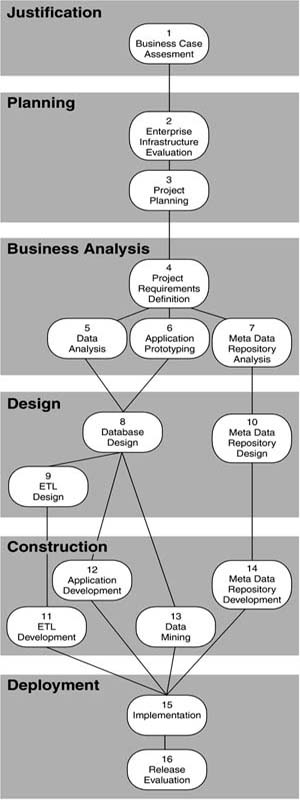
\includegraphics[width=0.4\textwidth]{fotos/11.png}
\caption{La curva negra indica la frontera de decisión KNN en los datos de la figura \ref{fig:2.13}, usando $K = 10$. La frontera de decisión de Bayes se muestra como una línea discontinua púrpura. Las fronteras de decisión KNN y de Bayes son muy similares.}
\label{fig:2.15}
\end{figure}

\begin{figure}[H]
\centering
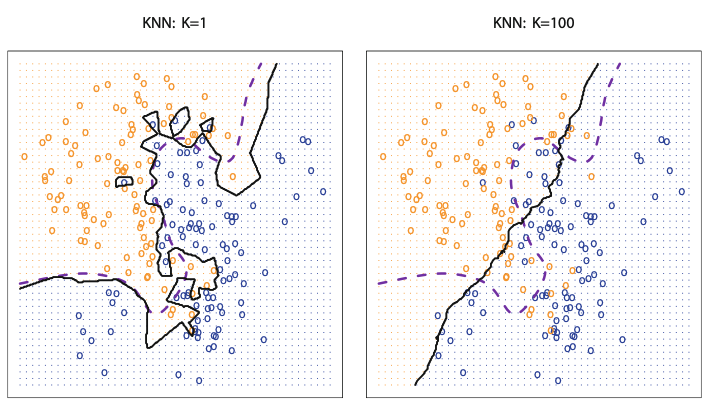
\includegraphics[width=0.7\textwidth]{fotos/12.png}
\caption{Una comparación de las fronteras de decisión KNN (curvas negras sólidas) obtenidas usando $K = 1$ y $K = 100$ en los datos de la figura \ref{fig:2.13}. Con $K = 1$, la frontera de decisión es excesivamente flexible, mientras que con $K = 100$ no es suficientemente flexible. La frontera de decisión de Bayes se muestra como una línea discontinua púrpura.}
\label{fig:2.16}
\end{figure}

La elección de $K$ tiene un efecto drástico en el clasificador KNN obtenido. La figura \ref{fig:2.16} muestra dos ajustes KNN a los datos simulados de la figura \ref{fig:2.13}, usando $K = 1$ y $K = 100$. Cuando $K = 1$, la frontera de decisión es excesivamente flexible y encuentra patrones en los datos que no corresponden a la frontera de decisión de Bayes. Esto corresponde a un clasificador que tiene bajo sesgo pero muy alta varianza. A medida que $K$ crece, el método se vuelve menos flexible y produce una frontera de decisión que es casi lineal. Esto corresponde a un clasificador de baja varianza pero alto sesgo. En este conjunto de datos simulado, ni $K = 1$ ni $K = 100$ dan buenas predicciones: tienen tasas de error de prueba de 0.1695 y 0.1925, respectivamente. \\

Al igual que en el contexto de regresión, no hay una relación estrecha entre la tasa de error de entrenamiento y la tasa de error de prueba. Con $K = 1$, la tasa de error de entrenamiento de KNN es 0, pero la tasa de error de prueba puede ser bastante alta. En general, a medida que se usan métodos de clasificación más flexibles, la tasa de error de entrenamiento disminuirá pero la tasa de error de prueba puede no hacerlo. En la figura \ref{fig:2.17} se han graficado los errores de prueba y de entrenamiento de KNN como una función de $1/K$. A medida que $1/K$ aumenta, el método se vuelve más flexible. Como en el contexto de regresión, la tasa de error de entrenamiento disminuye consistentemente a medida que aumenta la flexibilidad. Sin embargo, el error de prueba exhibe una forma característica de U, disminuyendo al principio (con un mínimo en aproximadamente $K = 10$) antes de aumentar nuevamente cuando el método se vuelve excesivamente flexible y sobreajusta. \\

En ambos contextos, de regresión y clasificación, elegir el nivel correcto de flexibilidad es crítico para el éxito de cualquier método de aprendizaje estadístico. El equilibrio entre sesgo y varianza, y la resultante forma de U en el error de prueba, pueden hacer de esta una tarea difícil. 

\begin{figure}[H]
\centering
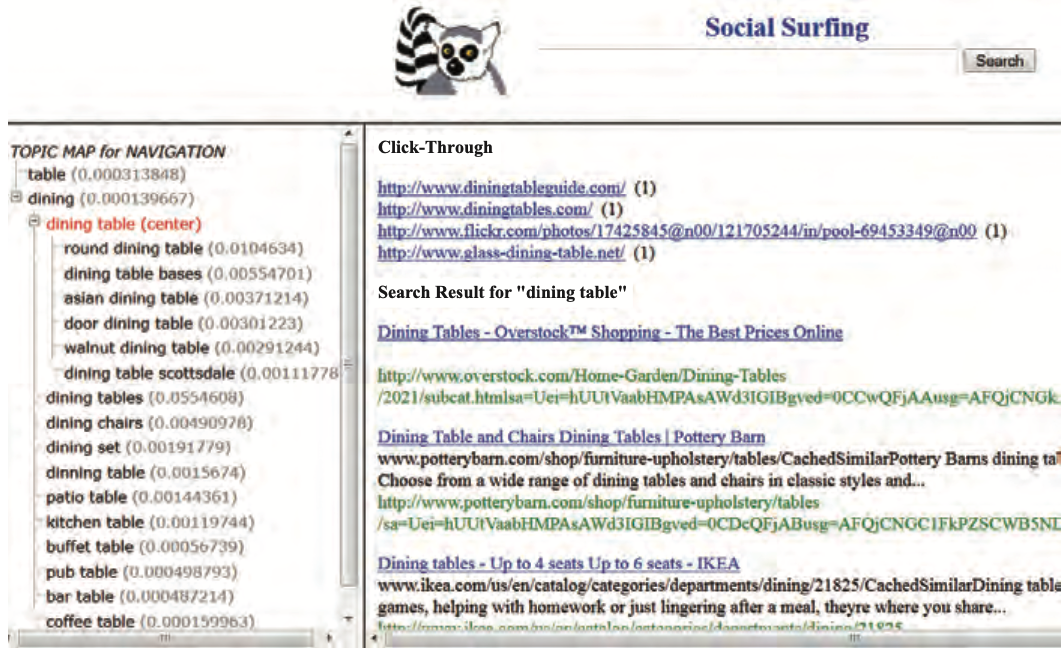
\includegraphics[width=0.6\textwidth]{fotos/13.png}
\caption{La tasa de error de entrenamiento KNN (azul, 200 observaciones) y la tasa de error de prueba (naranja, 5,000 observaciones) en los datos de la figura \ref{fig:2.13}, a medida que el nivel de flexibilidad (evaluado usando $1/K$) aumenta, o equivalentemente, a medida que el número de vecinos $K$ disminuye. La línea discontinua negra indica la tasa de error de Bayes. La irregularidad de las curvas se debe al pequeño tamaño del conjunto de datos de entrenamiento.}
\label{fig:2.17}
\end{figure}